% TEMPLATE for Usenix papers, specifically to meet requirements of
%  USENIX '05
% originally a template for producing IEEE-format articles using LaTeX.
%   written by Matthew Ward, CS Department, Worcester Polytechnic Institute.
% adapted by David Beazley for his excellent SWIG paper in Proceedings,
%   Tcl 96
% turned into a smartass generic template by De Clarke, with thanks to
%   both the above pioneers
% use at your own risk.  Complaints to /dev/null.
% make it two column with no page numbering, default is 10 point

% Munged by Fred Douglis <douglis@research.att.com> 10/97 to separate
% the .sty file from the LaTeX source template, so that people can
% more easily include the .sty file into an existing document.  Also
% changed to more closely follow the style guidelines as represented
% by the Word sample file. 

% Note that since 2010, USENIX does not require endnotes. If you want
% foot of page notes, don't include the endnotes package in the 
% usepackage command, below.

% This version uses the latex2e styles, not the very ancient 2.09 stuff.
\documentclass[letterpaper,twocolumn,10pt]{article}
\usepackage{usenix,epsfig,endnotes}
\begin{document}

%don't want date printed
\date{}

%make title bold and 14 pt font (Latex default is non-bold, 16 pt)
\title{\Large \bf Cross-platform Alternative to HomeOS}

%for single author (just remove % characters)
\author{
{\rm Christopher Becker}\\
University of Utah
\and
{\rm Shivam Kumar Sharma}\\
University of Utah
% copy the following lines to add more authors
% \and
% {\rm Name}\\
%Name Institution
} % end author

\maketitle

% Use the following at camera-ready time to suppress page numbers.
% Comment it out when you first submit the paper for review.
\thispagestyle{empty}


\subsection*{Abstract}
Networked ``smart home'' devices such as remotely controlled lights, cameras,
thermostats, and locks have become relatively inexpensive and widely available.
While, in theory, this should allow the proliferation of these devices as well
as the ability to use them in a wide range of scenarios such as adjusting the
climate control settings of a room based on occupancy levels or remotely
controlling a device such as a camera through a smart phone, in practice this is
not the case. The overhead of managing and extending the current systems is
generally not reasonable for any but expert hobbyists and the rich. As part of
the management of a system, access control is often difficult to correctly
configure, especially in systems with many devices and many users. This leads to
security and privacy issues which can result from misconfigured access control
rules.

Some recent work has been done to try to rectify this disparity by providing a
PC-like abstraction to easily manage and extend systems to include devices and
allow a wide range of scenarios. One specific system, HomeOS, was developed by
Microsoft Research. HomeOS is designed to be a system which presents devices as
peripherals, uses applications to allow cross-device tasks, provides a user
interface designed to be used in a home environment, and an easy to understand
access control system. However, HomeOS only runs on Windows.  We present an
alternative to HomeOS which provides cross-platform support.
\section{Introduction}
\label{sec:intro}
Networked ``smart home'' devices such as remotely controlled lights, cameras,
thermostats, and locks have become relatively inexpensive and widely available.
While, in theory, this should allow the proliferation of these devices as well
as the ability to use them in a wide range of scenarios such as adjusting the
climate control settings of a room based on occupancy levels or remotely
controlling a device such as a camera through a smart phone, in practice this is
not the case. The overhead of managing and extending the current systems is
generally not reasonable for any but expert hobbyists and the rich. As part of
the management of a system, access control is often difficult to correctly
configure, especially in systems with many devices and many users. This leads to
security and privacy issues which can result from misconfigured access control
rules.

Some recent work has been done to try to rectify this disparity by providing a
PC-like abstraction to easily manage and extend systems to include devices and
allow a wide range of scenarios. One specific system, HomeOS~\cite{homeOS}, was
developed by Microsoft Research. HomeOS is designed to be a system which
presents devices as peripherals, uses applications to allow cross-device tasks,
provides a user interface designed to be used in a home environment, and an easy
to understand access control system. However, HomeOS only runs on Windows.

We present an alternative to HomeOS which provides cross-platform support. Our
main contribution is providing a cross-platform system designed to have similar
capabilities as HomeOS which uses open source components. We also have made
minor changes to the system which we feel will improve the overall system.

The remainder of the paper is structured as follows: In
Section~\ref{sec:related} we introduce related work, focusing on HomeOS. In
Section~\ref{sec:arch} we provide an overview of the system architecture. In
Section~\ref{sec:implementation} we provide details about our implementation and
current status. We conclude with Section~\ref{sec:future} discussing future
work.
\section{Related Work}
\label{sec:related}
\subsection{HomeOS}
There is much research in this direction by Microsoft. HomeOS was developed by
Microsoft Research. Since the original system, Microsoft Research has continued
to use it for other research. Examples of this continued research are
HomeLab~\cite{homeLab} and Lab of Things~\cite{labOfThings}.

HomeLab is a shared infrastructure for conducting field studies for home
technology. HomeLab consists of a number of homes all containing different home
devices connected to PCs running HomeOS. A number of research groups can use
this infrastructure for conducting experiments on their device of interests.
HomeLab will allow easy sharing and co-ordination of research effort between the
different groups and will also allow them to focus on the actual experiment
rather than on the low level details of device connectivity etc. HomeLab also
allows groups to remotely update, monitor, and collect data from HomeOS.

Lab of Things consists of HomeOS and a number of cloud services. One of these
services is the Home Store from which a user can download drivers for different
devices.
\subsection{Access Control}

\section{Architecture}
\label{sec:arch}
\begin{figure}[tbh]
    \centering
    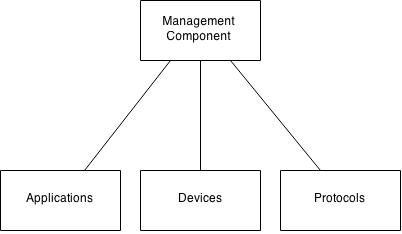
\includegraphics[width=1.0\columnwidth]{figs/homeOSArch.jpg}
    \caption{Architecture}
    \label{Fig:Arch}
\end{figure}
Figure~\ref{Fig:Arch} provides an overview of the architecture for our system.
Our system consists of four main components: Management Component, Applications,
Devices, and Protocols. The management component plays the central role of our
system. It handles the access control and communication between the other
components. All applications, devices, and protocols serve as modules and
fulfill roles. They use roles to communicate with each other. We will now
describe each component in more detail.
\subsection{Management Component}
\label{sec:mgmt}
The Management Component provides the core functionality and facilitates the
interactions within the system. The Management Component provides a user
interface for handling administrative tasks for the core system as well as
component management. Administrative tasks includes tasks such as user and
group setup and modification. Component Managment includes setting access
control rules for components, installing and uninstalling new components,
activating and deactivating installed components, and resolving dependencies
for components. 

When a component (other than the Management Component) wants to interact with
another component, it has to go through the Management Component. To the
Management Component, all other components are viewed as modules which are
described in more detail in Section~\ref{sec:mods}. When one component requests
to interact with another component, the Management Component first checks
against the access control rules before allowing the interaction to happen.
Access Control is described in more detail in Section~\ref{sec:access}.
\subsection{Applications}
\label{sec:apps}
\begin{figure}[tbh]                                                              
    \centering                                                                   
    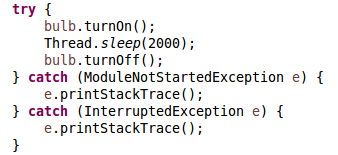
\includegraphics[width=1.0\columnwidth]{figs/appcode.png}                       
    \caption{Example application code snippet}                                  
    \label{Fig:appcode}                                                             
\end{figure} 
While the Management Component provides the core functionality of the system,
Applications provide functionality to the user. Applications facilitate
interactions between users and other components (besides the Management
Component). For instance, an application could turn on a light when a door is
unlocked.

The Applications are built as modules which are then are individually loaded
into the system. The Applications code is developed against our system.
Figure~\ref{Fig:appcode} shows a snippet of the code of the example application
that we developed. The application developer does not have to worry about which
protocol the light bulb uses to communicate, which manufacturer built that light
bulb, etc.
\subsection{Devices}
\label{sec:devices}
Devices provide interaction capability with the physical environment. Each
device is accessed through a device driver module which is loaded into the
system. These modules are also responsible for interacting with the
communication protocol modules. As described in Section~\ref{sec:protocols}.
Physical devices can include various types of sensors, light bulbs, door locks,
etc. Our device abstraction takes care of the heterogeneity that can exist with
the physical devices. Other parts of the system that communicate with Devices
don't have to worry about the lower level details regarding the actual physical
device.
\subsection{Protocols}
\label{sec:protocols}
Protocols provide an abstraction for communication protocols. These modules
allow device modules to interact with the physical devices. They also provide
the Management Component with information such as whether a physical device is
active or inactive or a new physical device is discovered.
\subsection{Modules}
\label{sec:mods}
A module is an interface that allows the Management Component to communicate
with the rest of the components in the system. All Applications, Devices, and
Protocols have to implement this interface. Every module has the capability to
start, stop, and tell the Management Component the list of roles (described in 
Section~\ref{sec:roles}) that they offer. Modules communicate with each
other through the use of roles.
\subsection{Roles}
\label{sec:roles}
A role is an interface that describes the functionality a module can provide. 
For example, a module implementing the ``light bulb'' role will provide functions
for turning on and off a light bulb. Roles play a critical role when two
modules interact. For example, if an application wants to turn on a light bulb,
the application requests a module that implements the ``"light bulb'' role from 
the Management Component. At this point, the Management Component searches for a
loaded module which implements that role and checks whether or not the
requesting module is allowed to access the module implementing the role. If the
Managment Component returns a module implementing that role, the application
then uses that returned module to turn on the light bulb.

\section{Implementation}
\label{sec:implementation}
The architecture discussed in Section~\ref{sec:arch} is implemented as a core
system, a user interface, and a set of modules. The system is written in Java.
\subsection{Core System}
\label{sec:core}
The core system is responsible for starting up the whole system. It first reads
the configuration file and establishes a connection with the data backend. The
core system is flexible as far as the backend is concerned and can communicate
with a variety of data backends including MySQL, Oracle, or flat files. The data
backend provides storage and lookup capabilities for user account informaton,
group information, access control information (as described in
Section~\ref{sec:access}), and component information. Once the connection to
the data backend has been established, the core system loads all the protocols,
devices, and applications modules in order. The core system contains an
Application Manager, Device Manager, and Protocol Manager to manage the various
types of components. It also keeps track of currently logged in users.
\subsection{Modules}
\label{sec:modules}
\begin{table}
\begin{center}
\begin{tabular}{| p{4cm} | p{3cm} |}
\hline
start() & Used by the Management Component to start the module \\ \hline
stop() & Used by the Management Component to stop the module \\ \hline
setModuleId() & Used by the Management Component to give the module an ID \\ \hline
getModuleId() & Used by the Management Component to get the ID of the module \\ \hline
getOfferedRoles() & Used by the Management Component to get the list of roles
offered by the module \\ \hline
serviceRegistered(roles) & Used by the Management Component to tell
the module that new roles are available \\ \hline
serviceDeRegistered(roles) & Used by the Management Component to tell
the module that some roles are no longer available \\ \hline
\end{tabular}
\end{center}
\caption{Module Interface}
\label{tab:module}
\end{table}

\begin{table}
\begin{center}
\begin{tabular}{| p{4cm} | p{3cm} |}
\hline
addModule() & adds a module to the system \\ \hline
removeModule() & removes a module from the system \\ \hline
getRole(String role) & Used by a module to request the ModuleManager to grant
access to a module offering the role sent as the parameter  \\ \hline
\end{tabular}
\end{center}
\caption{ModuleManager Interface}
\label{tab:modulemanager}
\end{table}
All applications, devices and protocols implement the Module interface. The
Module interface is required for a component to interact with the Management 
Component. Table~\ref{tab:module} provides an overview of the module interface.
Table~\ref{tab:modulemanager} provides an overview of the ModuleManager.
The ModuleManager is the part of the Management Component that interacts with
modules. Each module can offer some roles. Some modules might need specific
roles in order to fullfil their tasks. For example, an application (which is
also a module) that can turn on a light bulb would need a role called ``light
bulb.'' The application will ask the ModuleManager if there is a module that
offers the role ``light bulb.'' There can be another module, called
ZipatoLightBulb, that would be offering the role ``light bulb.'' If the
application has necessary permissions, the ModuleManger will allow the
application to interact with ZipatoLightBulb.
\subsection{User Interface}
\label{sec:interface}
\begin{figure}[tbh]                                                             
    \centering                                                                  
    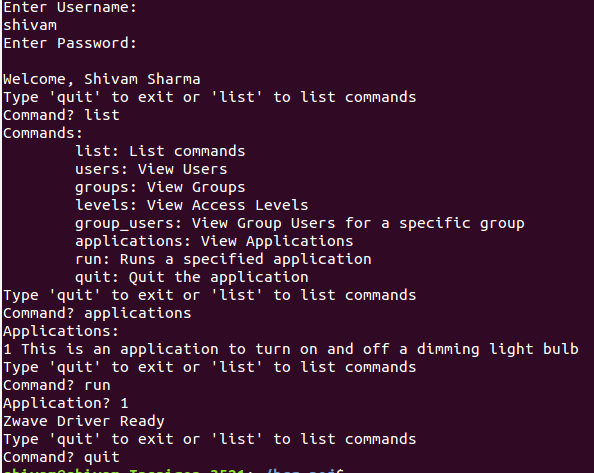
\includegraphics[width=1.0\columnwidth]{figs/cli.png}                
    \caption{Command Line Interface Screenshot}                                                      
    \label{Fig:cli}                                                            
\end{figure}
\begin{figure}[tbh]                                                             
    \centering                                                                  
    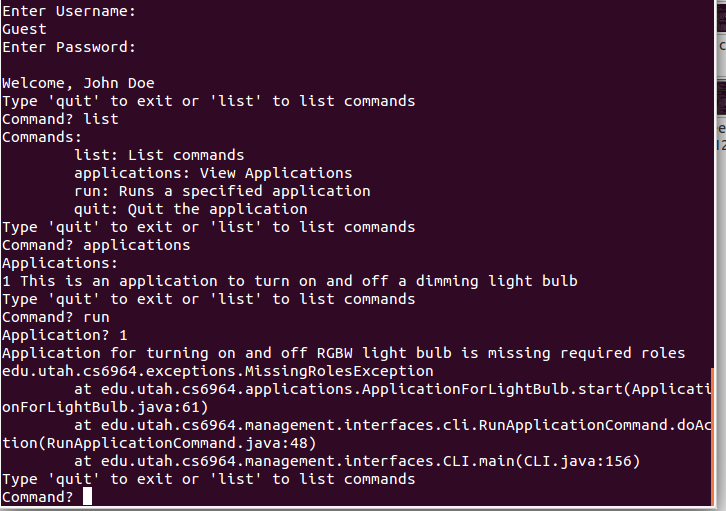
\includegraphics[width=1.0\columnwidth]{figs/cli2.png}                
    \caption{Command Line Interface Screenshot}                                                      
    \label{Fig:cli2}                                                            
\end{figure}
Currently, our system has a command line interface (CLI). We have designed the
user interface-related parts of our system in such a manner that replacing the
CLI with another interface in the future would be easily accomplished. The CLI
interacts with the core system to display information to the user and allow the
user to interact with the core system using a set of commands.

The CLI first asks the user to log in. Once the user has logged in, the CLI can
display a list of commands. The commands listed are based on the user's access
level (described in Section~\ref{sec:core_access}). Commands currently
implemented are: view users, view groups, view access levels, view users in
group, view applications, and run application.

Figure~\ref{Fig:cli} is a screenshot of the CLI for a user with access to all
commands. In the figure, after the user has logged in, he requests that the
system lists all commands available to him with the ``list'' command. Next, he
runs the ``applications'' command to view a list of currently available
applications (in this case our example application of turning a light bulb on
and off). Then, he runs our example application and quits. Whereas in
Figure~\ref{Fig:cli2} the user does not have permissions to view user and group
information. The user also does not have the permissions to run the example
application. Hence when the user tries to run it the system throws a
MissingRolesException.
\subsection{Access Control}
\label{sec:access}
Access control is divided into two types: core system access control and module
access control.
\subsubsection{Core System Access Control}
\label{sec:core_access}
The access control available for the core system (discussed in
Section~\ref{sec:core}) is designed to handle administrative tasks within the
core system. Users are divided into different levels of access. Currently, there
are eight levels of granularity, ranging from guests with minimal access to
full administrative users which have full permissions. Administrative tasks for
the core system include user account creation and modification, group creation
and assignment, and module access control administration.

Each user is assigned an access level, which is then used to determine which
commands the user can run. Each command is assigned a minimum access level.
When a user attempts to run the command, the access level of the user trying to
run the command is compared to the minimum access level of the command. If the
user's access level is greater than or equal to the minimum access level
assigned to the command, the user is able to run the command.
\subsubsection{Module Access Control}
Module access control provides access control between modules, which are
discussed in more detail in Section~\ref{sec:modules}. The access control
policies consist of a set of rules. Each rule consists of: a source module, a
destination module, the days of the week to which the rule applies, the start
and end times for those days, the user group to which the rule applies, the
priority of the rule, and the access mode.

When a user tries to use a module (either directly or indirectly), the system
looks for a rule that applies to the use. If a rule is found where the source
and destination modules match, then the system makes sure the current time and
day of the week match the rule and the user is part of the user group assigned
to the rule. The priority portion of the rule is used in the event of
conflicting access to the same module. The access mode can be either ``allow''
or ``ask.'' When the mode is ``allow,'' the interaction is automatically
allowed. When the mode is ``ask,'' a user is asked interactively to allow the
interaction at the time of access. Our system currently does not support the
priority or access mode portions of the rules.

Users are able to query the system to either figure out which modules a user can
access at a given time, based on the groups he or she is in, or figure out who
can access a given module. This allows the user to more reliably verify that the
access granted fits his or her expectations.

\section{Conceptual Differences from HomeOS}                                                           
\label{sec:homeosdiff}
As we were developing our system, several key changes from the original HomeOS
system were made which were either necessary or determined to be advantageous.
As a result of these differences, we are diverging from HomeOS. As we continue
with the development process, we expect to be significantly different from
HomeOS in the future.  We discuss the key changes in more detail below.
\subsection{Architectural Differences}
\label{sec:archdiff} 
\begin{figure}[tbh]                                                              
    \centering                                                                   
    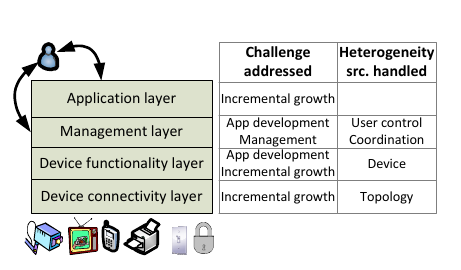
\includegraphics[width=1.0\columnwidth]{figs/homeosOrig.png}                     
    \caption{HomeOS Architecture from~\cite{homeOS}}                                 
    \label{Fig:homeosarch}                                                           
\end{figure}                                                                     
Figure~\ref{Fig:homeosarch} gives an overview of the original HomeOS
architecture taken from the HomeOS paper~\cite{homeOS}.
In the original HomeOS, the architecture of the system has been divided into 
stacked layers, with the application layer at the top. We decided that viewing
applications as components similar to devices and drivers was more intuitive.
This leads us to consider applications at the same level as the devices and
drivers, rather than a layer that sits on top of the management layer. This
leads the Management Component to play a more central and critical role.

HomeOS considers devices and protocols to fit under the same abstraction.
However, we view them as separate entities. We felt this was more intuitive and
might be more advantageous in the future.

Due to limitations with Java, all communication between components has to go
through the Management Component. This was a necessary change. This change has 
been discussed in more detail in the Section~\ref{sec:challenges}.
\subsection{Implementation Differences}
\label{sec:impldiff} 
One of the main differences between the original HomeOS system and our system is
that our system is written in Java rather than C\#. We chose to use Java to try
to maximize the cross-platform capabilities, as well as pull from a larger pool
of developers. We also strived to use only open source libraries to also improve
cross-platform support and encourage community-based development.

While the module access control, discussed in more detail in
Section~\ref{sec:module_access}, closely resembles the access control system
used by HomeOS, the core access control system is of our own design, discussed
in more detail in Section~\ref{sec:core_access}. In addition, while HomeOS used
datalog, we are using database tables to mimic the functionality of datalog.

We felt it was important to provide a flexible data backend and not tie our
system to one particular data storage system. The data backend must provide
certain functionality, but the actual implementation and storage format is left 
to the developer.

\section{Challenges}
\label{sec:challenges}
While developing the system we had to overcome a number of challenges. We have 
mentioned them below.

The first challange we faced was in installation of the drivers for the zwave
controller. The drivers were not compatible with our kernel version ( Ubuntu 
3.13.0-43-generic). We started modifying the existing driver source but 
eventually we were able to find drivers that had been modified to work with our
system.

The second challenge we faced was in building the Java wrappers for the
OpenZWave library. The build process for the Java wrappers requires the path to
the directory containing the source code for OpenZWave. If the OpenZWave
directory contains the source code as well as the binaries, the building of the
Java wrappers failed. After a lot of hit and trail we were luckily able to find
this out and fix it.

The third challenge we faced was in changing the color of the light bulb. The
OpenZWave library doesn't support that yet. We decided to write our own code to
do that. We were not able to find out the exact message that needs to be sent to
the bulb in order to change its color. The original Z-Wave library is
proprietary and there is no freely available documentation for it. Most of the 
OpenZWave library has been developed by reverse engineering and hit and trial.
The OpenZWave forum helped us here and told us that device needs to be sent an
RGB value to change its color. The exact byte sequence that needs to be sent
will contain the following
0x20x"Red color value"0x3"Green color value"0x4"Blue color value".

The last challenge was because of Java not allowing us to free memory on demand.
When ManagementComponent approves the request of Module1 to communicate with
Module2 it sends an instance of Module2 to the requesting instance of Module1.
In the original HomeOS paper if the ManagementComponent later decides to revoke
Module1's capability to access Module2 it simply frees the memory occupied by
the instance of Module2 this is something that we cannot do in Java. Hence we 
had to redesign our system and force all communication that can happen between
modules to go through the ManagementComponent.  

\section{Results and Future Work}
\label{sec:future}
Currently, our system only supports the Z-Wave protocol. We want
to add support for protcols such as Bluetooth, Wi-Fi, ZigBee, etc. We currently
have a device driver only for the Zipato RGBW light bulb. We would like to add
drivers for music players, thermostats, security cameras, motion detectors, etc.
This will allow us to create applications with richer functionality, like having
a light start blinking and starting a security camera when movement is detected
by a motion sensor. Currently, we have an application that can turn on and off a
light bulb.

Future work includes adding additional functionality and continuing to expand
the API available to users and developers, as well as making extension of the
system easier. We talk about this in more detail below.

We want to create an infrastructure that can allow the users to easily install
new components and roles. Similar to HomeOS, we envision having packages that
contain a Manifiest file and binaries. Our system will read the Manifest and
install the binaries accordingly.

We want to give the user the capability to specify per user defaults for
components. For example, if we have an application that can turn on the light
bulb and there are two light bulbs in the home, one in the living room and one
in the bedroom, currently the application will prompt the user to ask which
light bulb to use. Instead, the user could save that preference and the
application will use that component by default in the future.

We plan to improve and expand the access control mechanisms and improve the user
interface, to improve both the usability and security of the system. We plan on
having the capability to create time-based user accounts. For example, if the
owner has visitors coming over, the owner can create accounts that will be
active only during the duration of the stay of the visitors. Currently, we
cannot force the components to not access the file system or the network. We
want to add these security features to our system.

We wish to add an online marketplace, to allow users to easily find applications
and drivers to extend and improve their systems. Similarly, the developers can
upload their applications to the marketplace, allowing easy access to the users.

Lastly, we wish to create a more graphical and intuitive user interface which
will allow the user to easily extend, configure, and query the system.


{\footnotesize \bibliographystyle{acm}
\bibliography{biblio}}


%\theendnotes

\end{document}







 
